%!/usr/bin/env pdflatex
%-*- coding: utf-8 -*-
%@author : Romain Graux
%@date : 2022 Mar 08, 16:20:03
%@last modified : 2022 Mar 15, 13:35:12


% [ PLAN ] 
% - Motivation
%   - Classical compressors (JPEG, ...)
%   - What we need (tasks)
%   - What they built
% - Intuition
%   - Example on MNIST

\documentclass[8pt,t]{beamer}


% Import all packages
\usepackage{graphicx,caption}

% Color declarations
\definecolor{greyBackgroundColor}{rgb}{0.8,0.8,0.8}
\definecolor{primaryColor}{rgb}{0.5,0,0.5}
\definecolor{secondaryColor}{rgb}{0,0,0}

% Theme definition and progessbar settings
\usetheme[progressbar=frametitle]{metropolis}
\setbeamertemplate{frame numbering}[fraction]

% Settings of all colors
\setbeamercolor{background canvas}{bg=white}
\setbeamercolor{title}{fg=primaryColor}
\setbeamercolor{frametitle}{bg=greyBackgroundColor, fg=primaryColor}
\setbeamercolor{structure}{fg=primaryColor}
\setbeamercolor{subsection in head/foot}{fg=secondaryColor}
\setbeamercolor{progress bar}{fg=secondaryColor}

% Personal commands declaration
\newcommand{\docsPath}[1]{./docs/#1}
\newcommand{\imgsPath}[1]{\docsPath{imgs/#1}}

% Meta information declaration
\title{Lossy compression for lossless prediction}
\subtitle{EECS Seminar: Advanced Topics in Machine Learning}
\author{Romain Graux}
\date{\today}

\begin{document}

\begin{frame}
    \titlepage
\end{frame}

\begin{frame}{Motivation}
    $10^{21}$ - $10^{23}$ bytes data collected per year

    \only<2->{
        $\rightarrow$ But most data is processed by algorithms performing \textbf{downstream tasks}.
    \vspace{5pt}
    }

    \def \imgWidth {0.23\textwidth}

    \only<3>{
        \begin{figure}
            \centering
            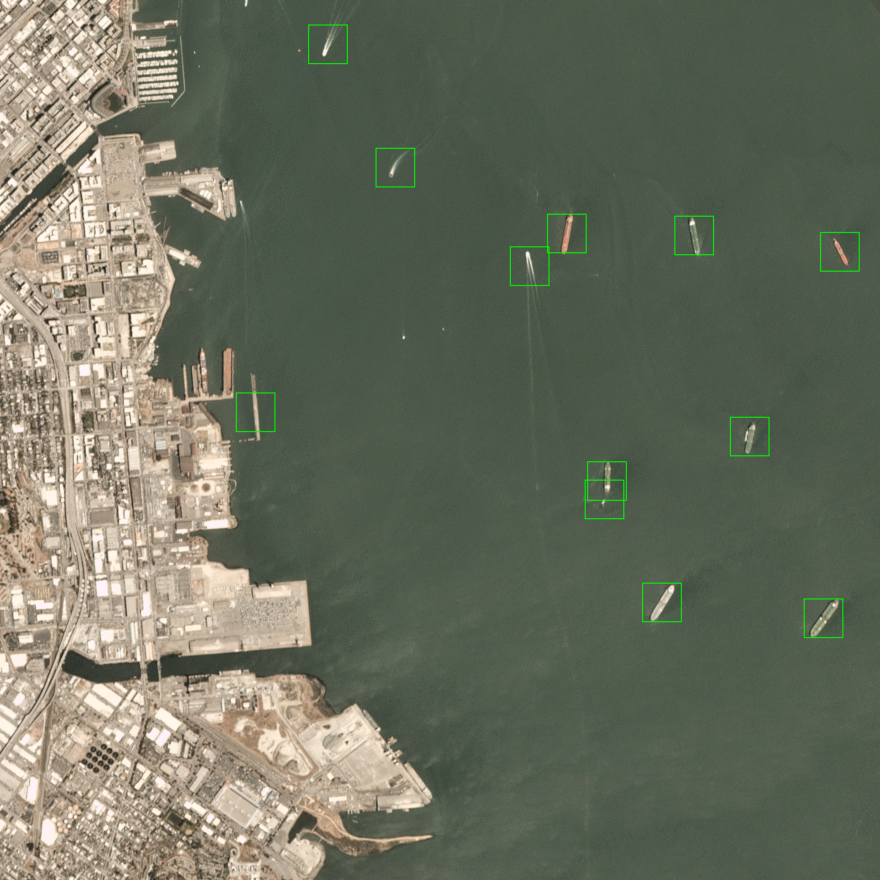
\includegraphics[width=\imgWidth]{\imgsPath{applications/satellite-detection.png}} \quad
            \includegraphics[width=\imgWidth]{\imgsPath{void.png}} \\
            \includegraphics[width=\imgWidth]{\imgsPath{void.png}} \quad
            \includegraphics[width=\imgWidth]{\imgsPath{void.png}} 
        \end{figure}
    }

    \only<4>{
        \begin{figure}
            \centering
            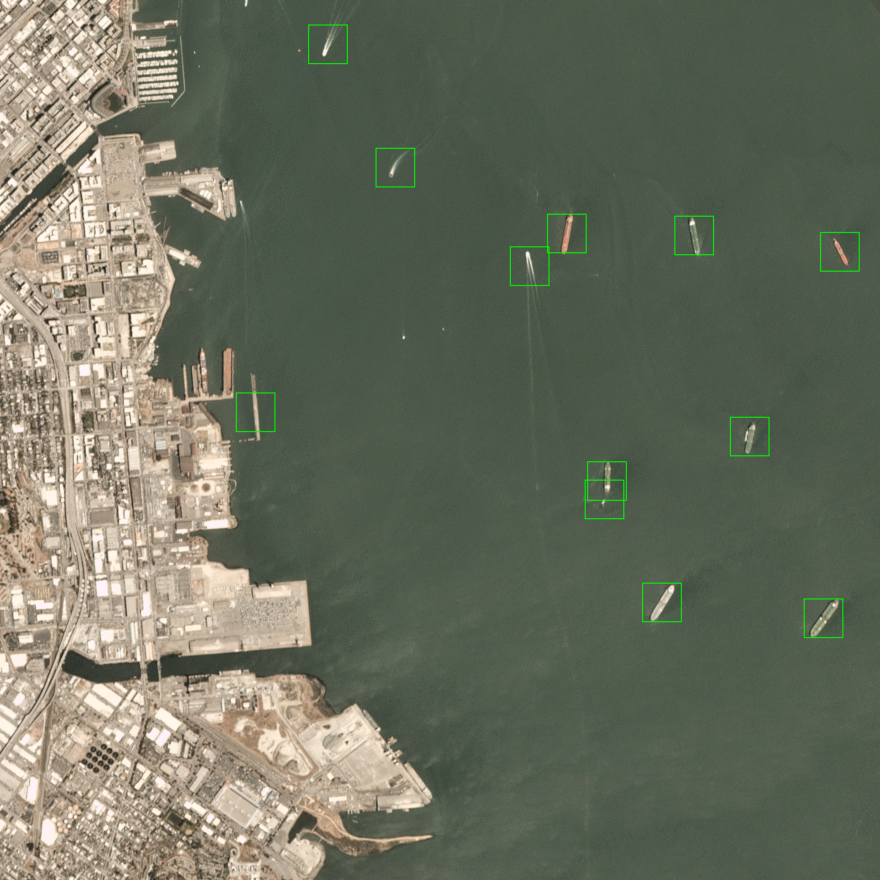
\includegraphics[width=\imgWidth]{\imgsPath{applications/satellite-detection.png}} \quad
            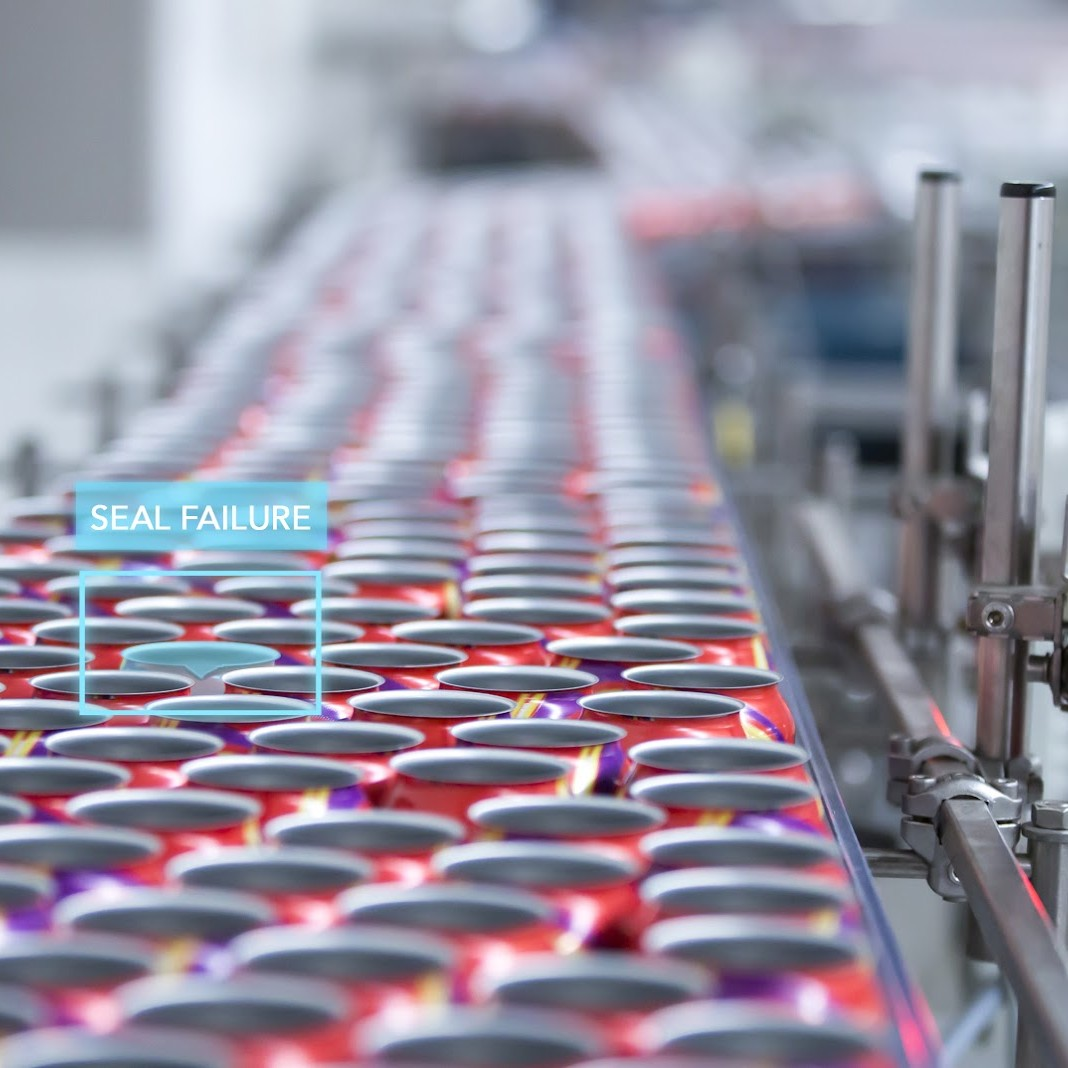
\includegraphics[width=\imgWidth]{\imgsPath{applications/quality_control.jpg}} \\
            \includegraphics[width=\imgWidth]{\imgsPath{void.png}} \quad
            \includegraphics[width=\imgWidth]{\imgsPath{void.png}} 
        \end{figure}
    }

    \only<5>{
        \begin{figure}
            \centering
            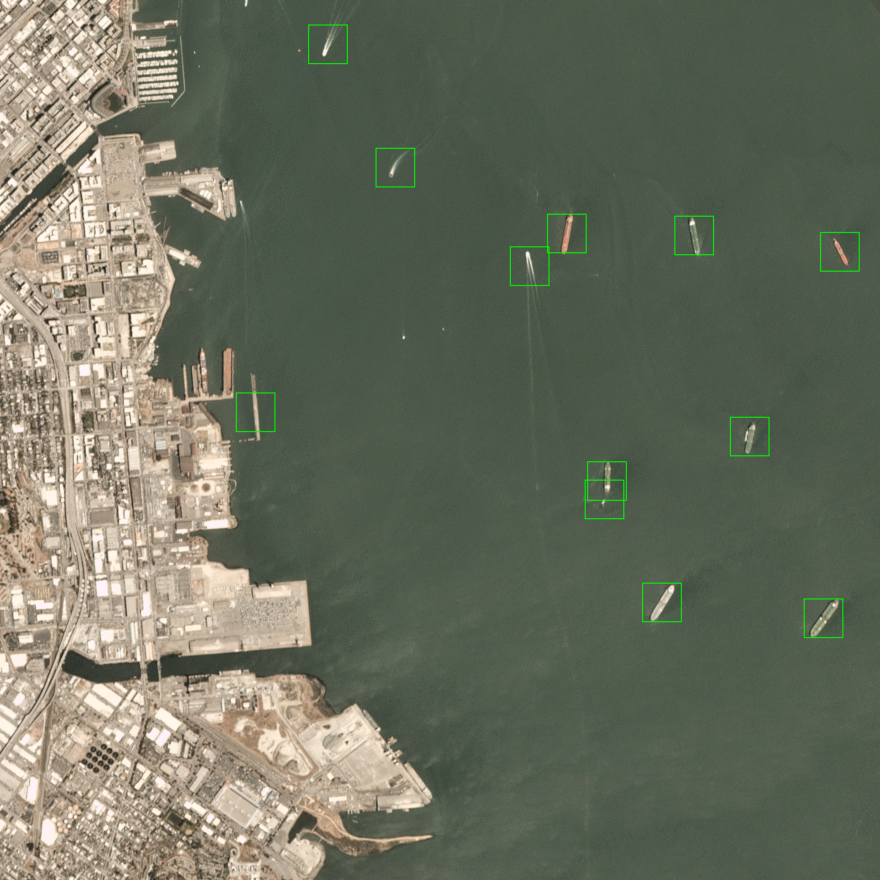
\includegraphics[width=\imgWidth]{\imgsPath{applications/satellite-detection.png}} \quad
            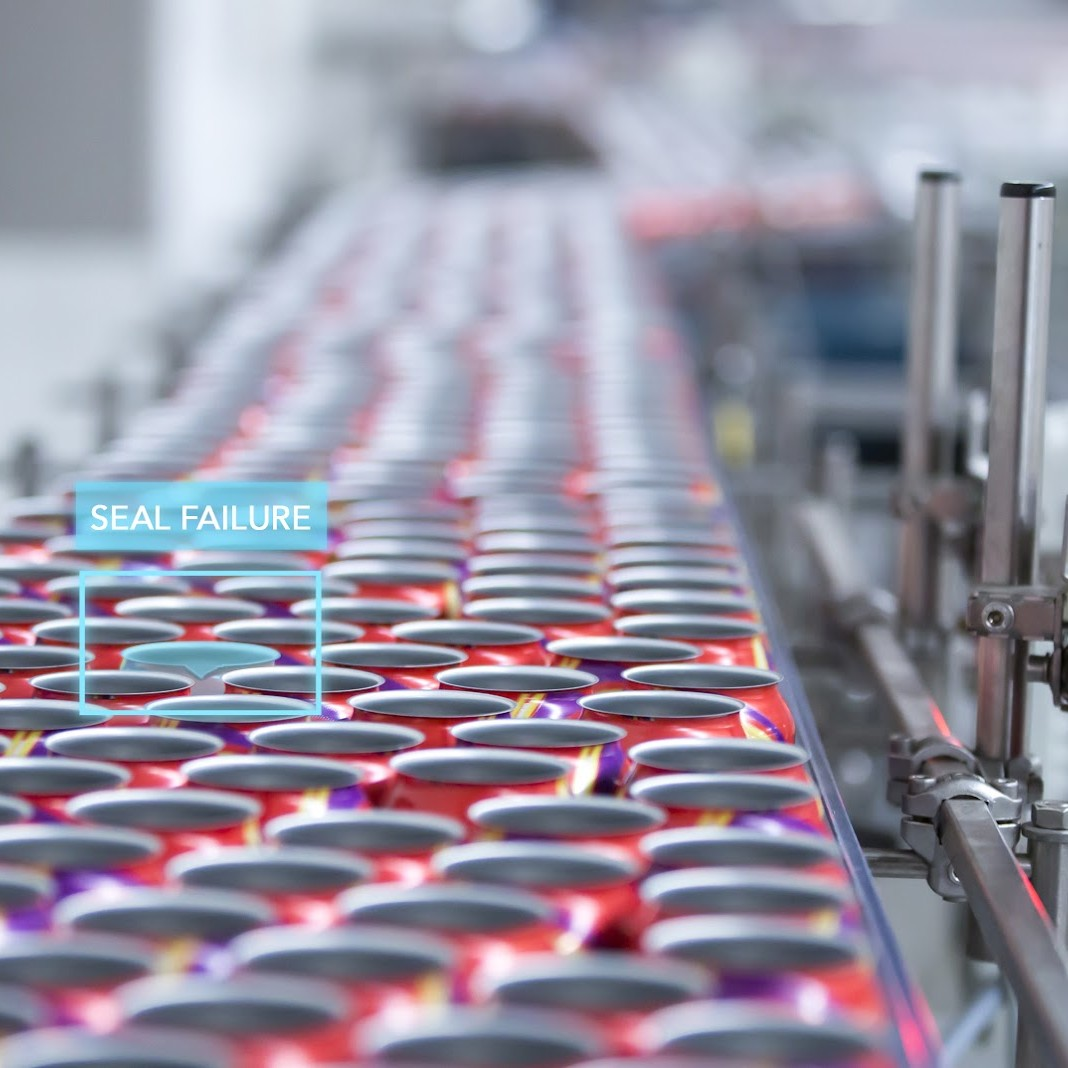
\includegraphics[width=\imgWidth]{\imgsPath{applications/quality_control.jpg}} \\[12pt]
            \includegraphics[width=\imgWidth]{\imgsPath{void.png}} \quad
            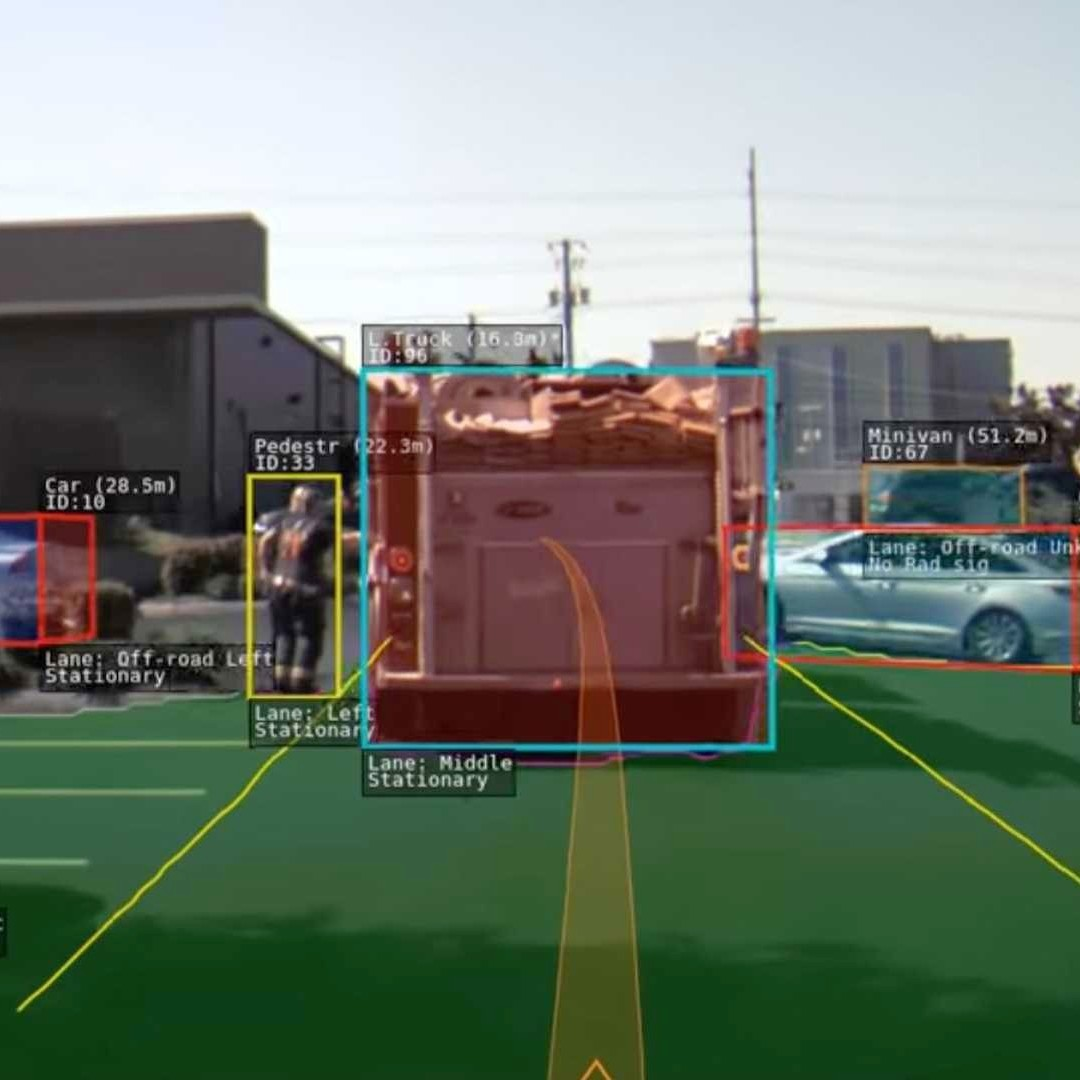
\includegraphics[width=\imgWidth]{\imgsPath{applications/selfdriving-cars.jpeg}} 
        \end{figure}
    }

    \only<6>{
        \begin{figure}
            \centering
            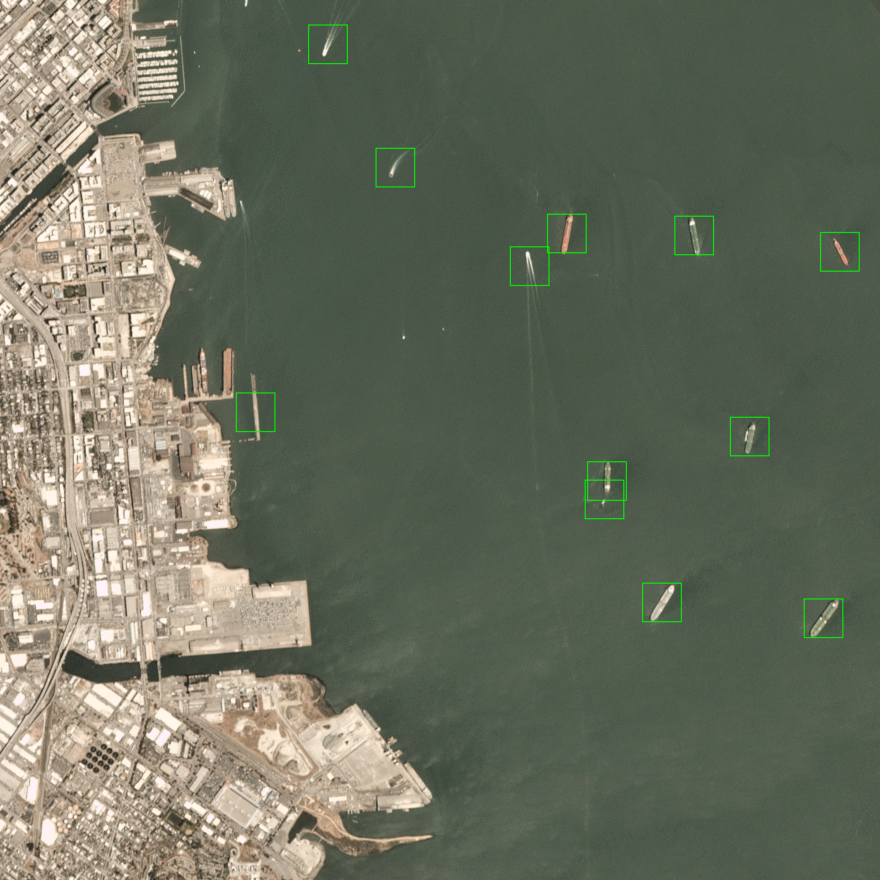
\includegraphics[width=\imgWidth]{\imgsPath{applications/satellite-detection.png}} \quad
            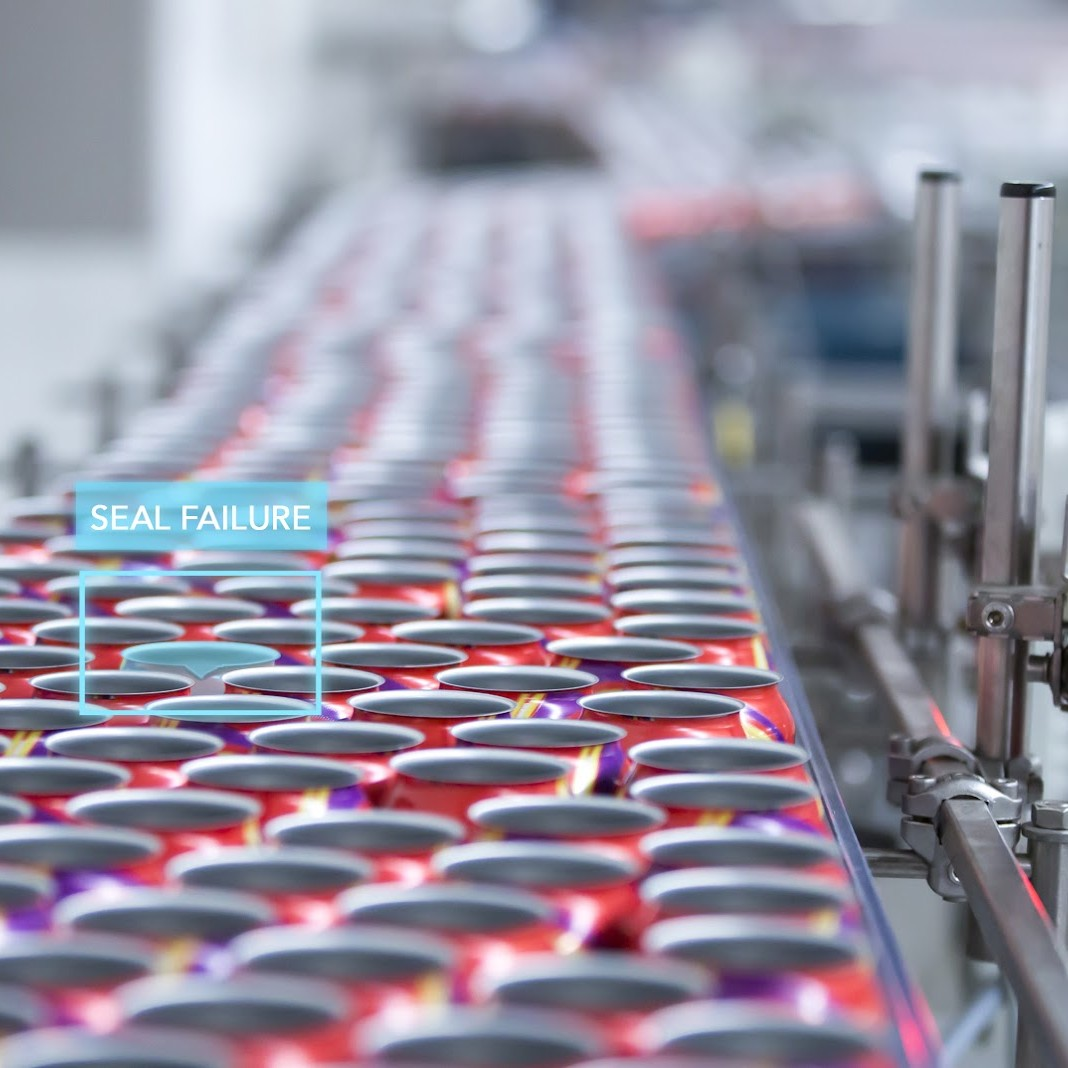
\includegraphics[width=\imgWidth]{\imgsPath{applications/quality_control.jpg}} \\[12pt]
            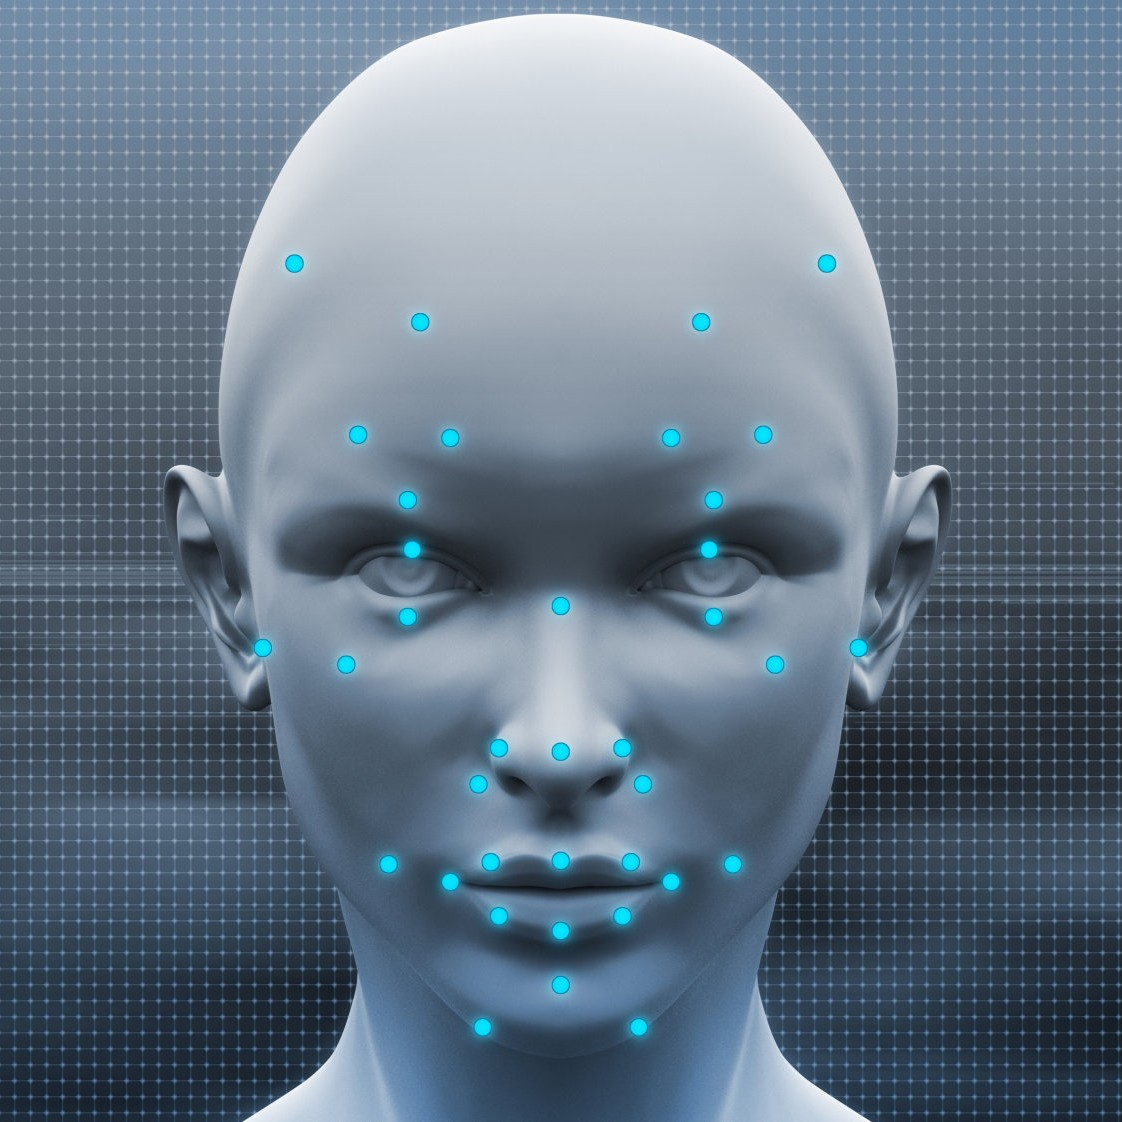
\includegraphics[width=\imgWidth]{\imgsPath{applications/face-recognition.jpeg}} \quad
            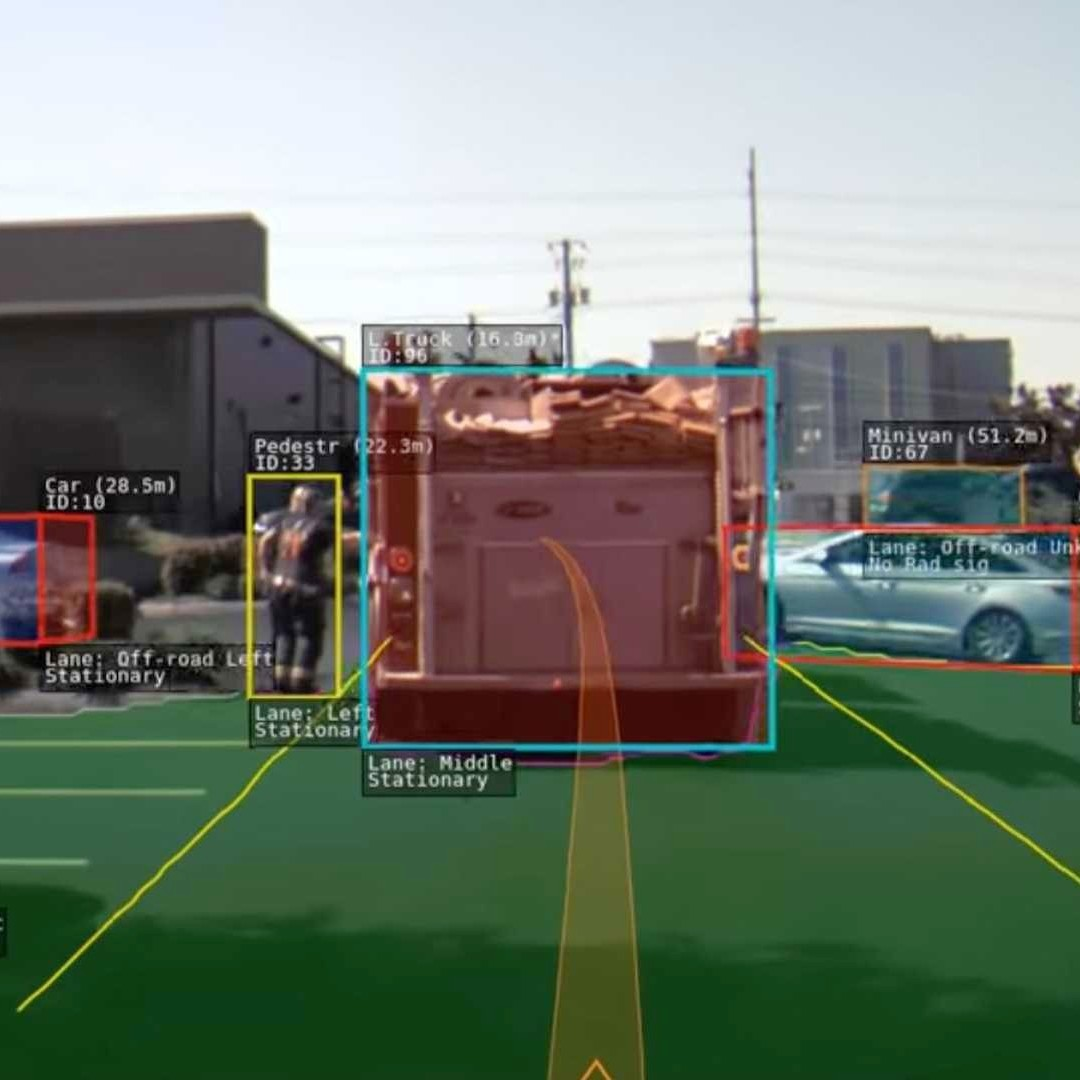
\includegraphics[width=\imgWidth]{\imgsPath{applications/selfdriving-cars.jpeg}} 
        \end{figure}
    }

    \only<7->{
        Yet current compressors optimize high \textbf{perceptual} fidelity
    }

    \only<8->{
        \begin{itemize}
            \item Stores too much not needed information
            \item Does not ensure good task performance
        \end{itemize}
    }


    \vfill
    \begin{columns}
    \column{0.2\textwidth}
    \only<9->{
            \begin{figure}
                \centering
                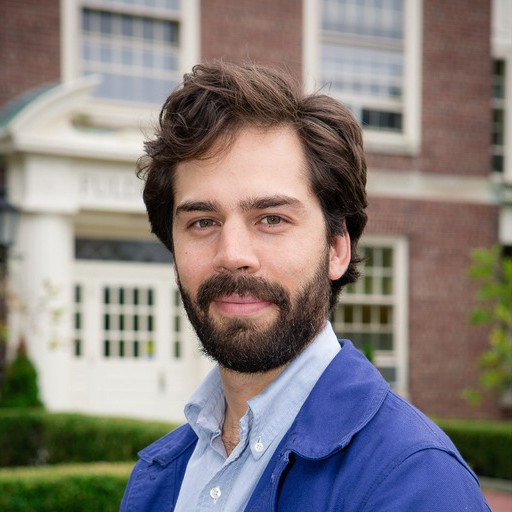
\includegraphics[width=\textwidth]{\imgsPath{chris/source.jpeg}}
                \caption*{Source}
                \label{fig:chris-source}
            \end{figure}
    }

    \column{0.2\textwidth}
    \only<10->{
            \begin{figure}
                \centering
                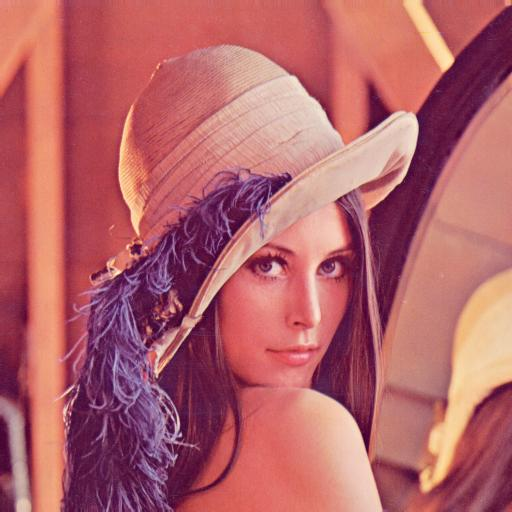
\includegraphics[width=\textwidth]{\imgsPath{chris/high.jpeg}}
                \caption*{High bitrate}
                \label{fig:chris-high}
            \end{figure}
    }

    \column{0.2\textwidth}
    \only<11->{
            \begin{figure}
                \centering
                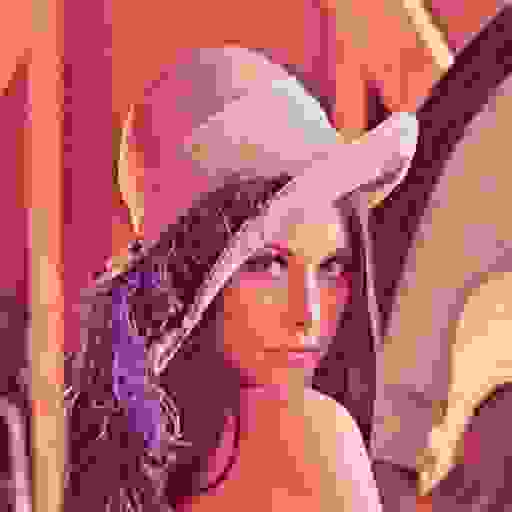
\includegraphics[width=\textwidth]{\imgsPath{chris/low.jpeg}}
                \caption*{Low bitrate}
                \label{fig:chris-low}
            \end{figure}
    }

    \column{0.2\textwidth}
    \only<12->{
            \begin{figure}
                \centering
                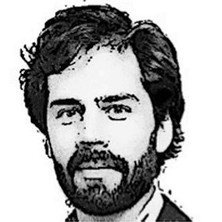
\includegraphics[width=\textwidth]{\imgsPath{chris/desired.jpeg}}
                \caption*{Desired}
                \label{fig:chris-desired}
            \end{figure}
    }
    \end{columns}


    % \def \imgWidth {0.2\textwidth}

    % \only<8->{
    %     \begin{figure}
    %         \centering
    %         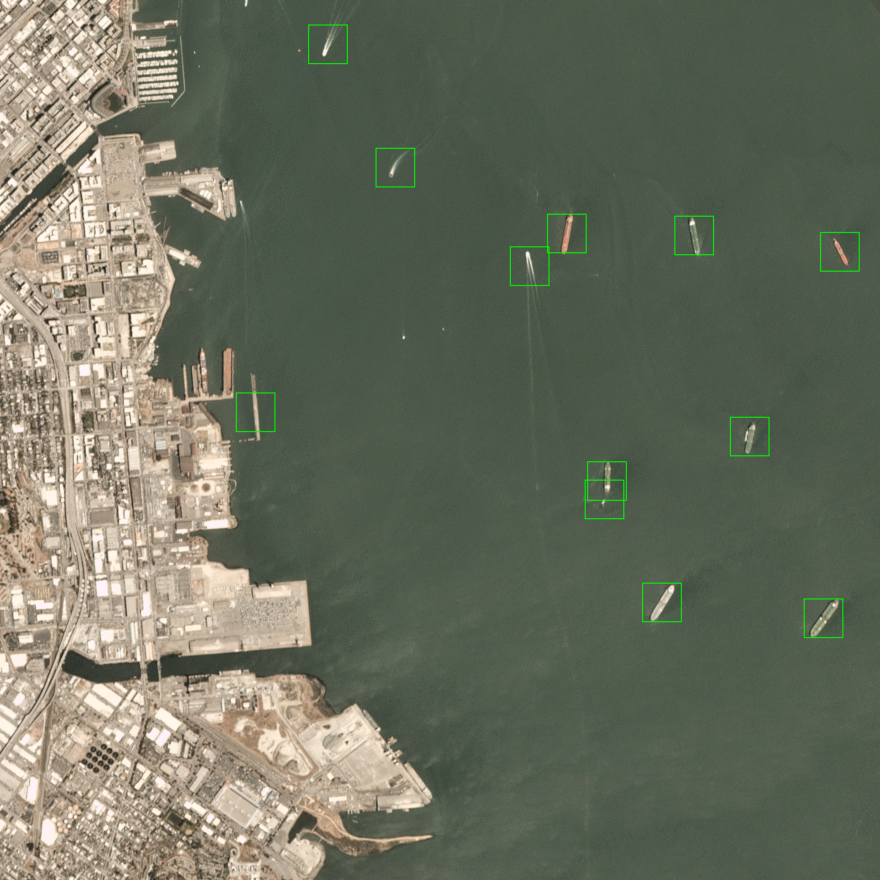
\includegraphics[width=\imgWidth]{\imgsPath{applications/satellite-detection.png}} \quad
    %         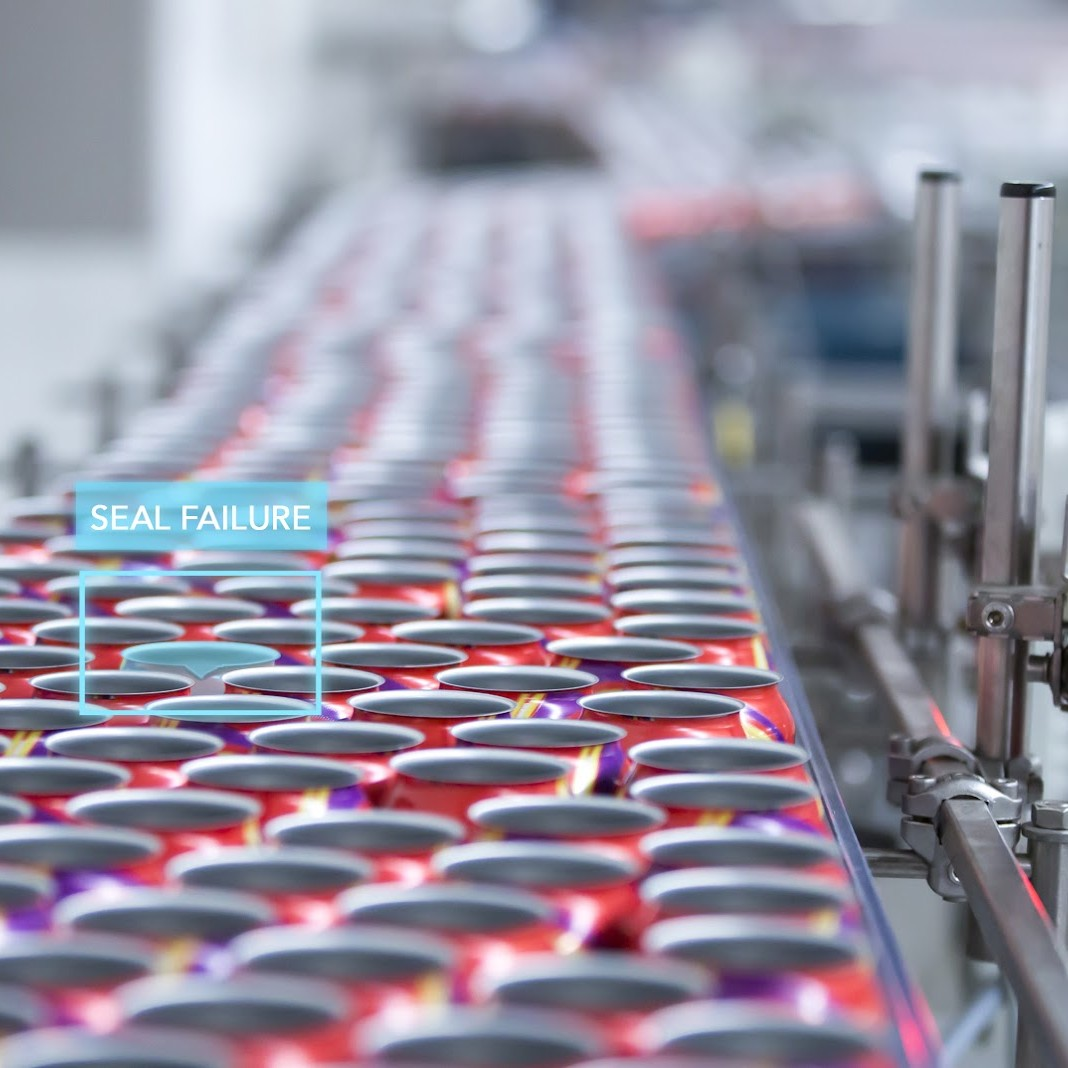
\includegraphics[width=\imgWidth]{\imgsPath{applications/quality_control.jpg}} \quad
    %         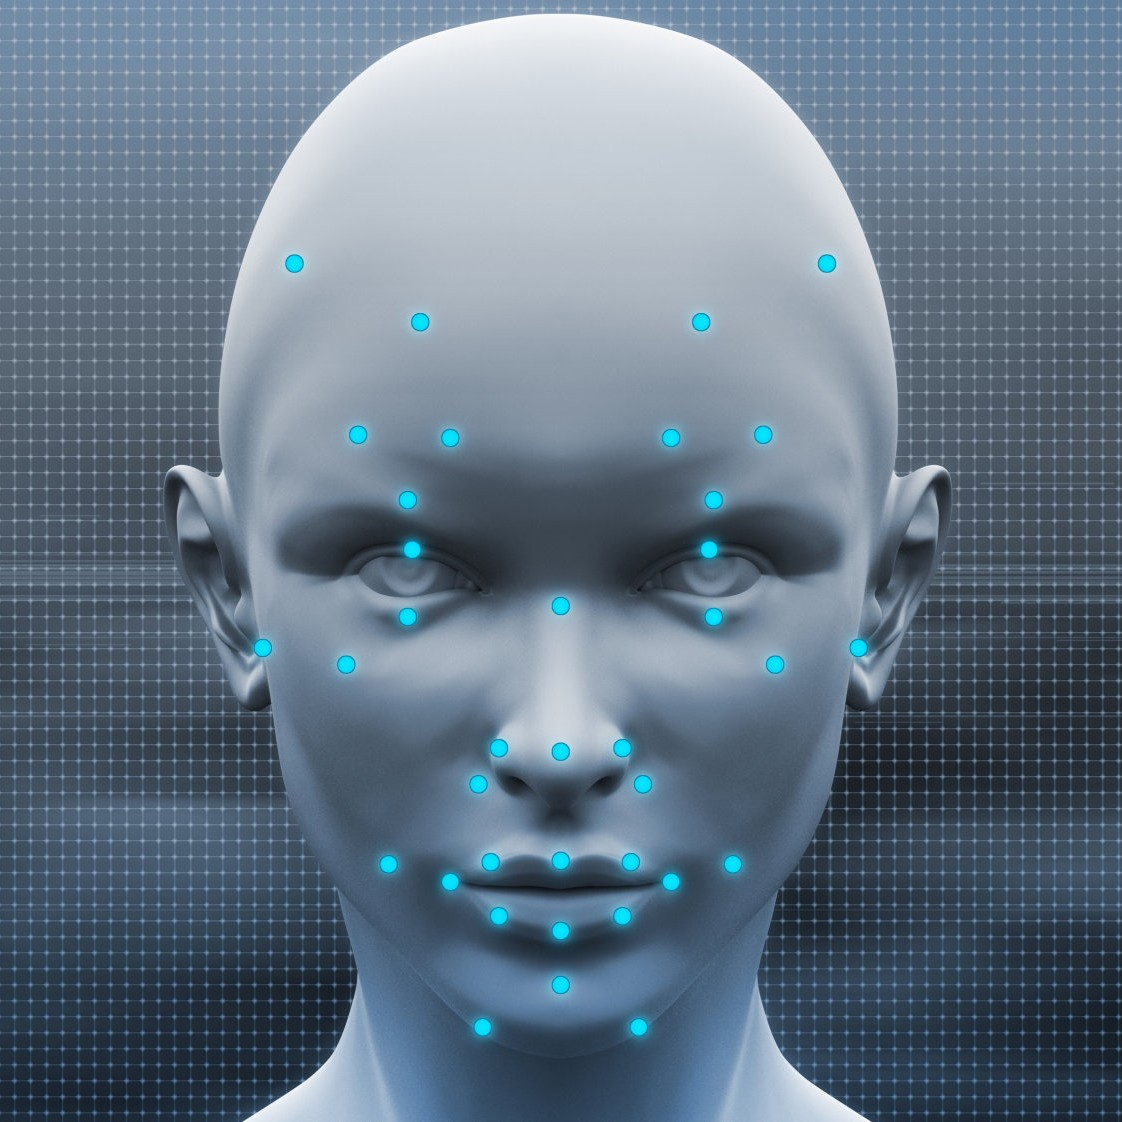
\includegraphics[width=\imgWidth]{\imgsPath{applications/face-recognition.jpeg}} \quad
    %         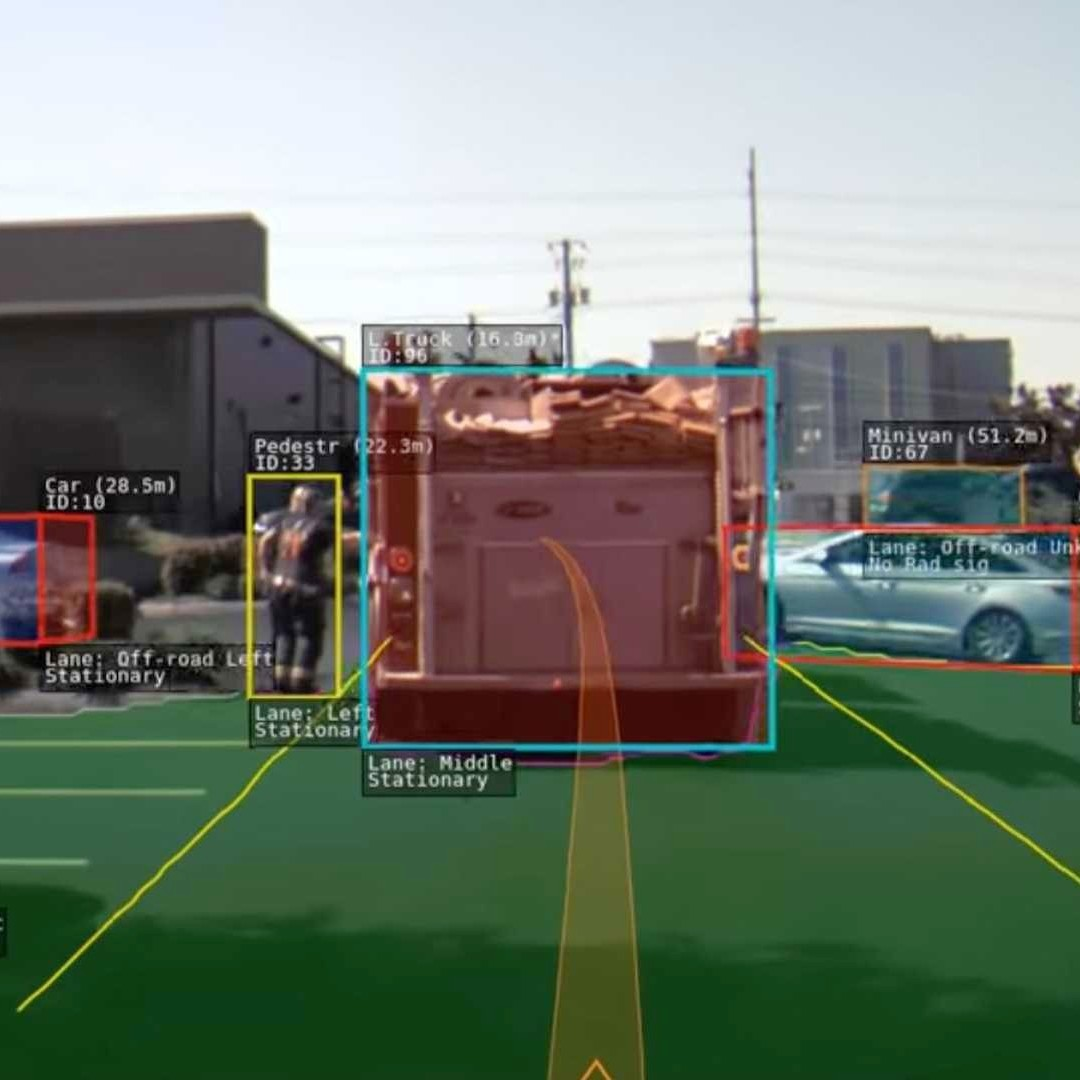
\includegraphics[width=\imgWidth]{\imgsPath{applications/selfdriving-cars.jpeg}} 
    %     \end{figure}
    % }


\end{frame}

\end{document}

